\chapter{Implementação e resultados}
\label{cap:implementacaoresultados}

Neste capítulo será detalhado a implementação, com a configuração do \ac{OS}, do ambiente virtualizado e das ferramentas que irão compôr o
\textit{cluster} de alta disponibilidade. Posteriormente, serão efetuados testes e medições de resultados.

Nas próximas seções será demonstrado a configuração das ferramentas do ambiente de alta disponibilidade, do ambiente de virtualização e 
também do sistema operacional.

Descrever o que nao deu certo no projeto com o ganeti??

\section{Topologia}

A estrutura física adotada está representada na Figura \ref{fig:projeto_fisico}.

\begin{figure}[h!]
 \centering
 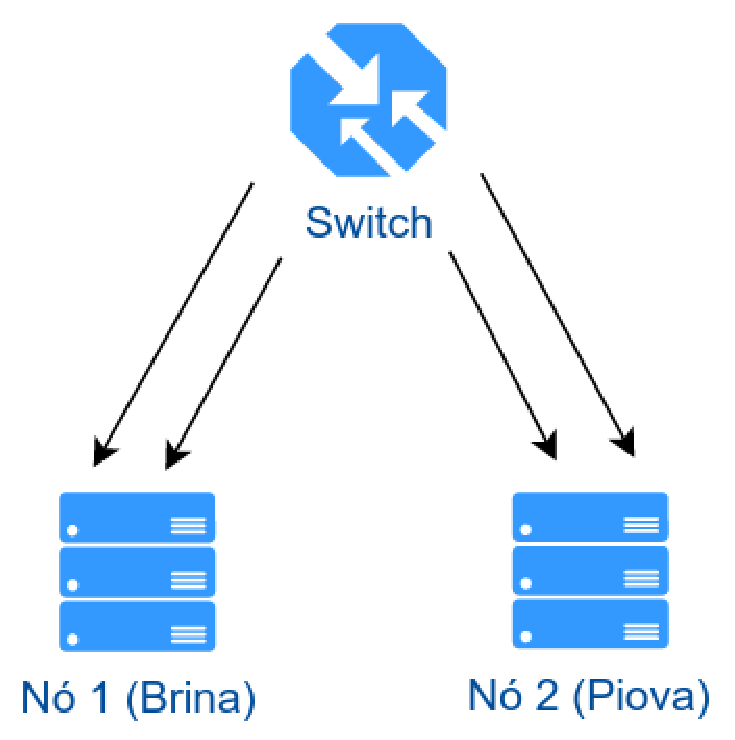
\includegraphics[width=180px]{img/projeto_fisico.eps}
 \caption{Estrutura física.}
 \label{fig:projeto_fisico}
\end{figure}

Pode-se observar os dois servidores ligados a um \textit{switch} através de dois cabos UTP cada servidor ...

Na Figura \ref{fig:servidores_brina_piova} tem-se a imagem dos servidores, o primeiro no topo da imagem, \textit{Brina} 
(\textit{Dell PowerEdge 2950}), e o servidor mais abaixo, \textit{Piova} (\textit{Dell PowerEdge R410}).

\begin{figure}[h!]
 \centering
 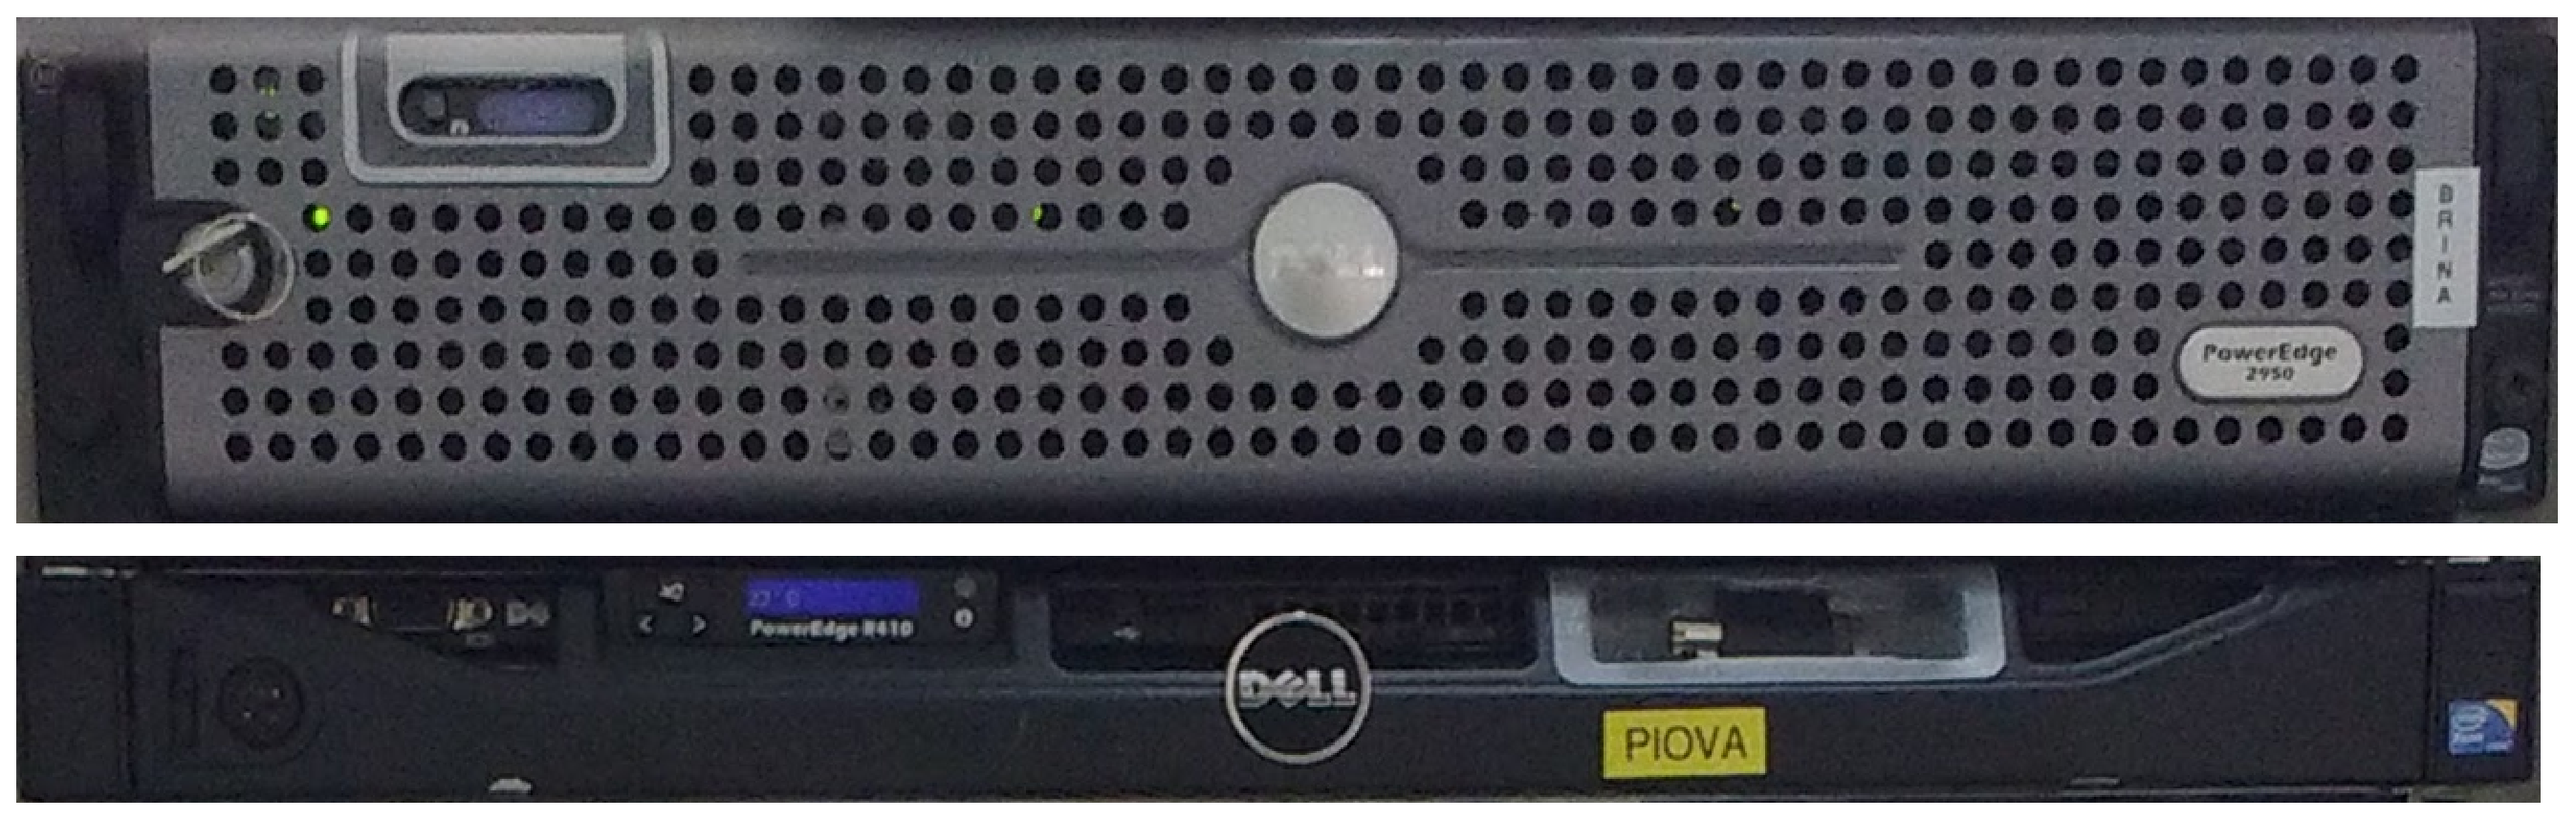
\includegraphics[width=300px]{img/servidores_brina_piova.eps}
 \caption{Servidores.}
 \label{fig:servidores_brina_piova}
\end{figure}

Pode ser observado na Figura \ref{fig:projeto_estrutura} a estrutura que representa a configuração dos \textit{softwares}. Nesta tem-se o 
\textit{software} de gerenciamento do cluster, que fará o monitoramento, iniciará e parará os recursos dos nós, o \textit{software} de replicação 
de dados, o sistema de arquivos, as máquinas virtuais e os serviços localizados nestas máquinas.

\begin{figure}[h!]
 \centering
 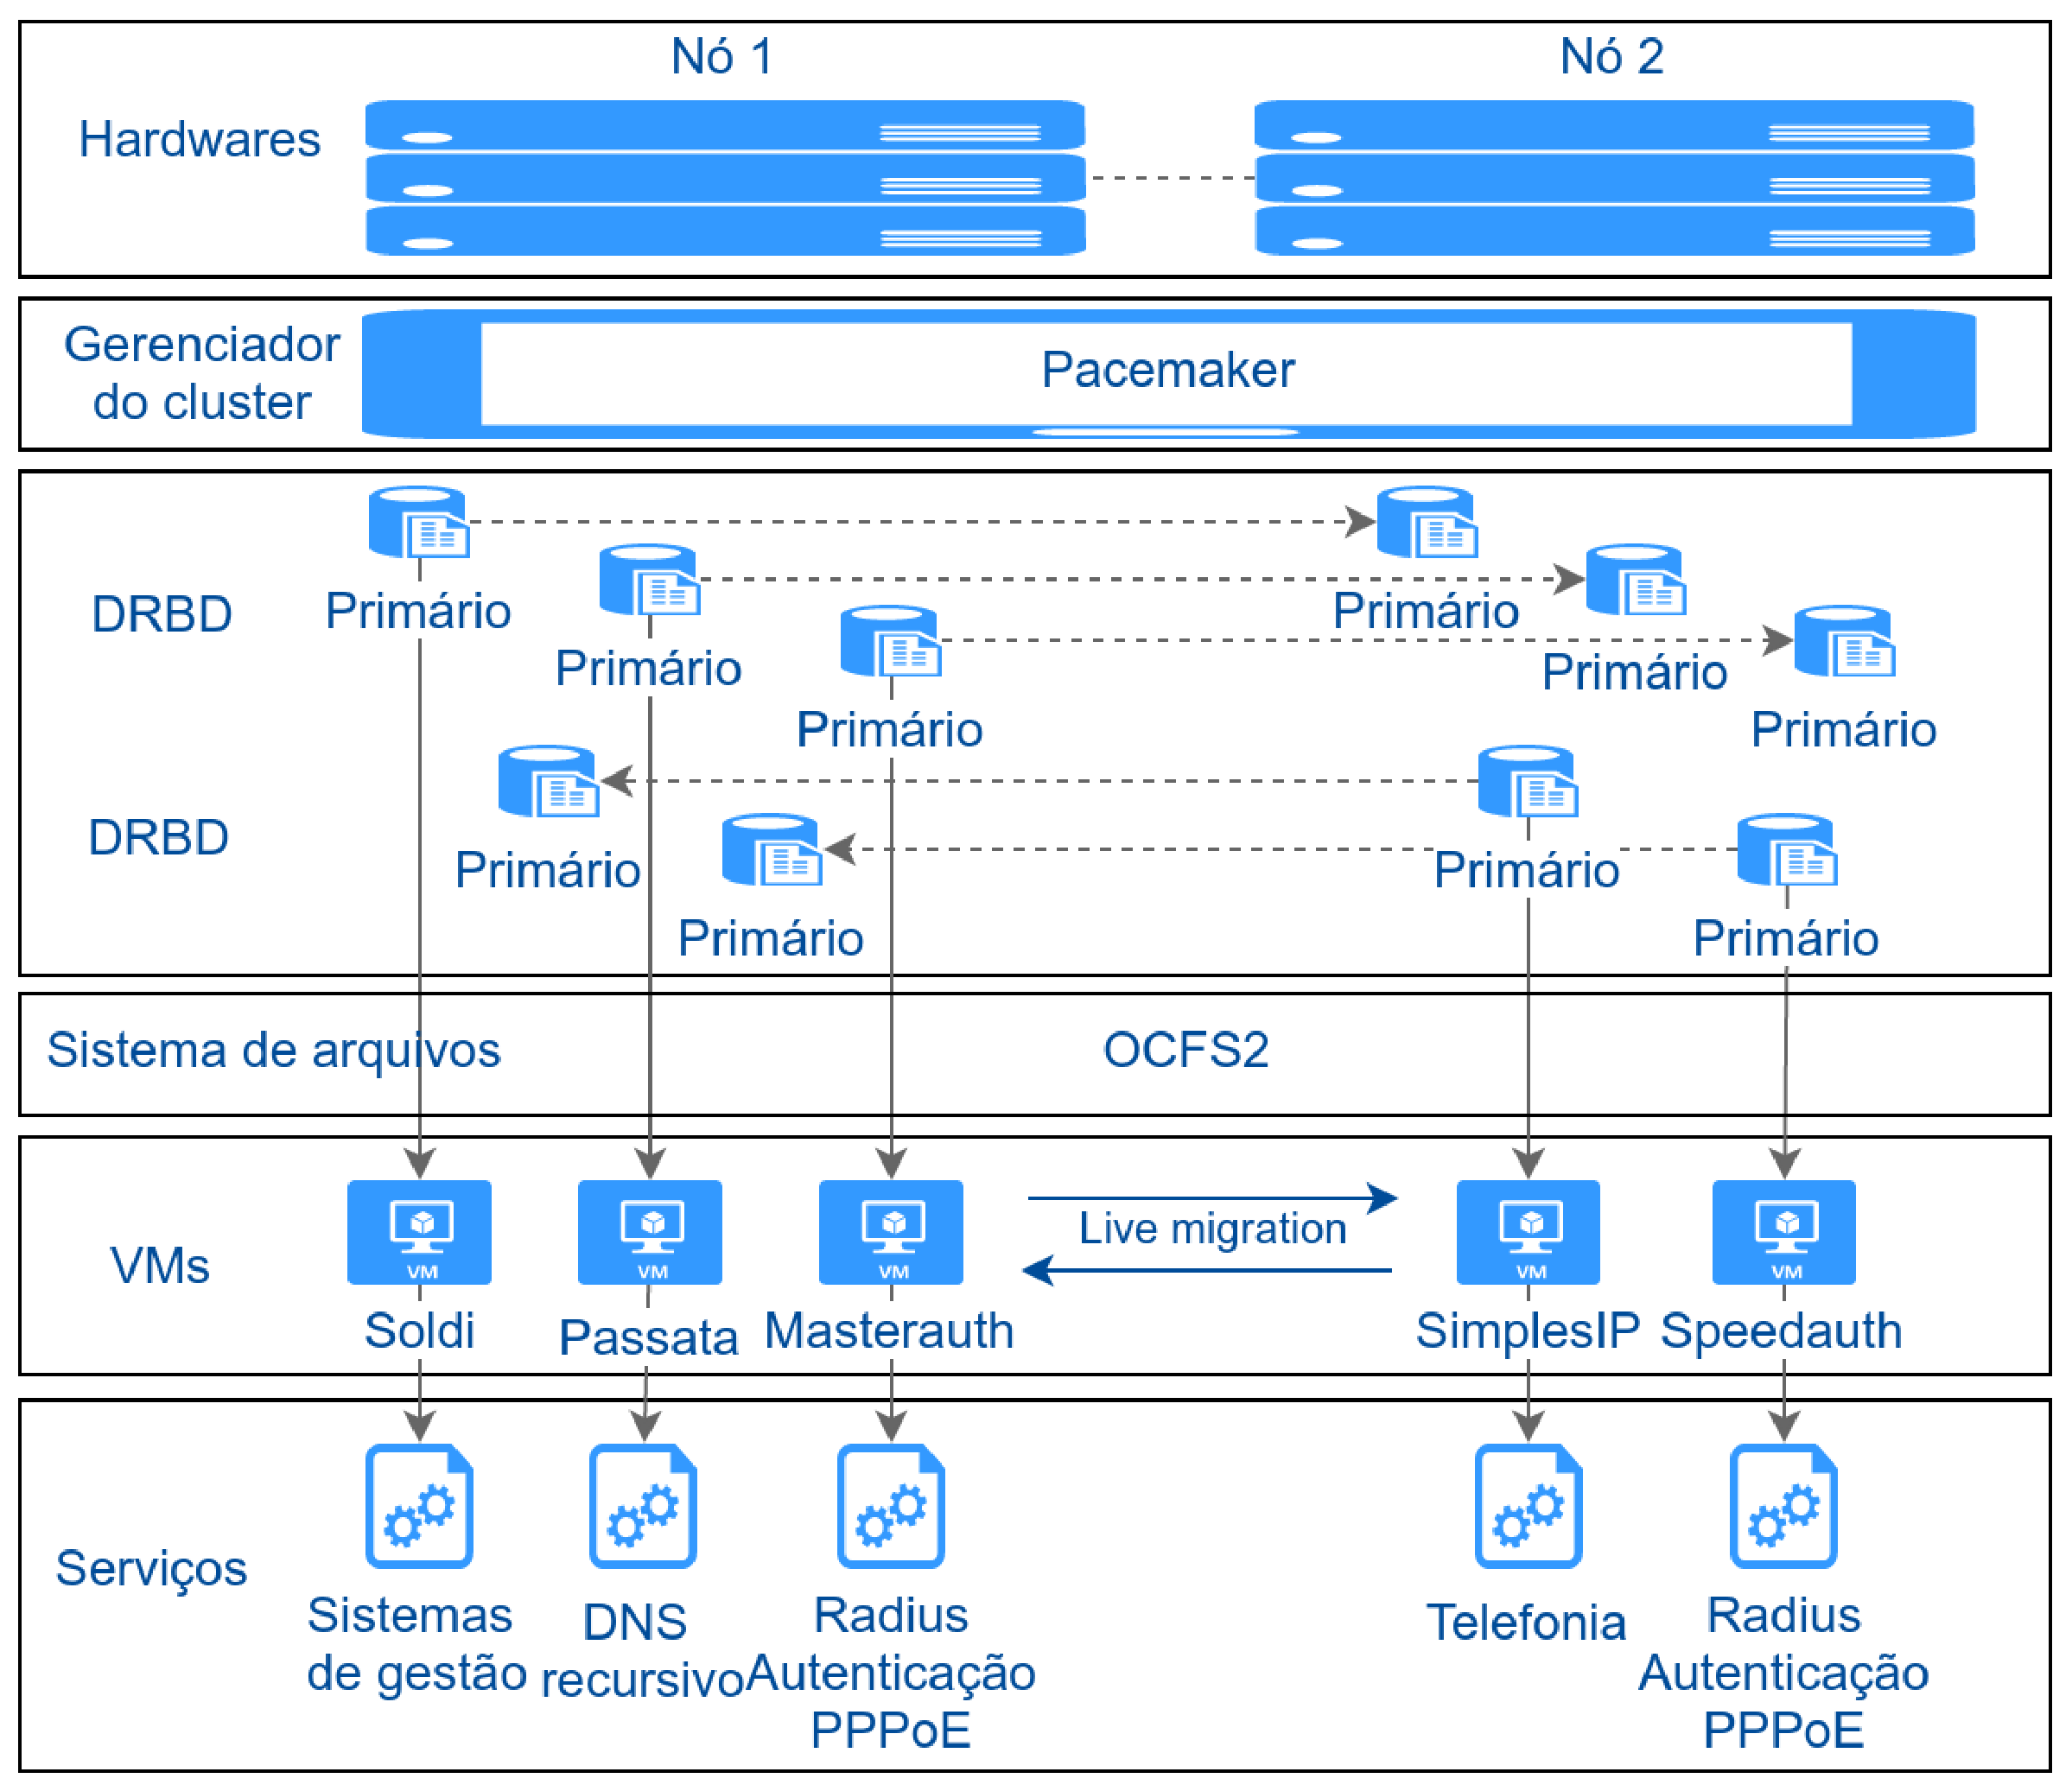
\includegraphics[width=350px]{img/projeto_estrutura.eps}
 \caption{Estrutura do \textit{cluster}.}
 \label{fig:projeto_estrutura}
\end{figure}

tabela com ips??

\section{Configuração do \ac{OS}}

Foi feita a instalação do sistema operacional \textit{Ubuntu 14.04 \ac{LTS}} nos dois servidores. A configuração feita foi a básica do sistema,
com nome do servidor, configuração de rede, localização e instalação do servidor \ac{SSH}.
Além disso, é feito as configurações padrões adotadas pela empresa, como por exemplo, ferramentas de monitoramento, atualização automática
e \textit{firewall}.

\section{Configuração de rede}

Um requisito para incluir as máquinas virtuais a uma rede é através da criação de uma \textit{bridge}. A instalação é feita através do comando:
\begin{lstlisting}[language=bash]
  $ apt-get install bridge-utils
\end{lstlisting}

Além disso, é necessário instalar e configurar o \textit{link aggregation}, padrão adotado foi o ??. A configuração é feita no servidor e 
no \textit{switch}. Abaixo tem-se os comandos para instalação do \textit{link aggregation}, o primeiro comando faz a instalação
e o segundo comando carrega o modulo do \textit{kernel} \textit{bonding}:
\begin{lstlisting}[language=bash]
 $ apt-get install ifenslave-2.6
 $ sh -c 'grep -q bonding /etc/modules || echo bonding >> /etc/modules'
\end{lstlisting}

Para a configuração do \textit{link aggregation} deve-se criar uma interface \textit{bond} e nela inclui-se as duas interfaces físicas.
Abaixo tem-se a configuração de rede, que inclui o \textit{link aggregation} e a \textit{bridge}, esta configuração deve ser colocada no 
arquivo \textit{/etc/network/interfaces}:
\begin{lstlisting}[language=bash]
auto eth0
iface eth0 inet manual
bond-master bond0

auto eth1
iface eth1 inet manual
bond-master bond0

auto bond0
iface bond0 inet manual
       bond-mode 4
       bond-slaves eth0 eth1
       bond-lacp-rate 1
       bond-miimon 100
       bond-xmit_hash_policy layer3+4

auto br0
iface br0 inet static
       address x.x.x.x
       netmask 255.255.255.0
       network x.x.x.0
       broadcast x.x.x.255
       gateway x.x.x.x
       dns-nameservers 8.8.8.8 8.8.4.4
       
       bridge_ports bond0
       bridge_stp off
       bridge_maxwait 0
\end{lstlisting}

\section{Configuração de disco}

Os discos que serão replicados podem ser utilizados diretamente no \ac{DRBD} (por exemplo \textit{/dev/sda2}) ou configurados com \ac{LVM}. Adotou-se
a configuração utilizando \ac{LVM} pois torna-se mais fácil a manipulação dos discos. O comando abaixo faz a criação de um volume lógico chamado 
\textit{lvdrbd} com tamanho de 500 GB, este volume pertence ao grupo de volumes \textit{vg0}.
\begin{lstlisting}[language=bash]
 $ lvcreate -n lvdrbd vg0 -L 500G
\end{lstlisting}

\subsection{DRBD}

Para a instalação do \textit{software} de replicação de dados é necessário instalar os dois pacotes, que estão listados abaixo:
\begin{lstlisting}[language=bash]
 $ apt-get install drbd8-utils drbdlinks
\end{lstlisting}

É necessário alterar a configuração global do \ac{DRBD} que está localizada em \textit{/etc/drbd.d/global\_common.conf}:
\begin{lstlisting}[language=bash]
global {
        usage-count yes;
        minor-count 16;
}
\end{lstlisting}

Posteriormente, deve-se criar um recurso que definirá os dispositivos de disco, os endereços \ac{IP} e portas dos servidores.
Deve-se criar o arquivo \textit{/etc/drbd.d/vms.res}, o qual armazenará essa configuração:
\begin{lstlisting}[language=bash]
 resource vms {
    meta-disk internal;
    device /dev/drbd0;
    protocol C;
    disk {
        fencing resource-only;
        resync-rate 50M;
    }
    handlers {
        fence-peer "/usr/lib/drbd/crm-fence-peer.sh";
        after-resync-target "/usr/lib/drbd/crm-unfence-peer.sh";
    }
    net {
        allow-two-primaries;
    }
    startup {
        become-primary-on both;
    }
    on brina {
        address x.x.x.x:7791;
        disk /dev/vg0/lvdrbd;
    }
    on piova {
        address x.x.x.x:7791;
        disk /dev/vg0/lvdrbd;
    }
    syncer {
        rate 50M;
    }
}
\end{lstlisting}
Explicar os parametros??

Para o funcionamento correto dessa ferramenta, o nome dos servidores (localizado em \textit{/etc/hostname}) deve ser exatamente igual ao parâmetro
\textit{on} da configuração do recurso.

...

\section{Configuração do ambiente virtualizado}

chaves ssh root??

\section{Configuração do cluster}


\subsection{Pacemaker}

